\documentclass[screen, aspectratio=169]{beamer}
\usepackage[T1]{fontenc}
%\usepackage[utf8]{inputenc}

% Use the NTNU-temaet for beamer 
% \usetheme[style=ntnu|simple|vertical|horizontal, 
%     language=bm|nn|en, 
%     smalltitle, 
%     city=all|trondheim|alesund|gjovik]{ntnu2017}
\usetheme[style=ntnu,language=en]{ntnu2017}

\usepackage[english]{babel}
\usepackage[style=numeric,backend=biber,natbib=false,sorting=none]{biblatex}

\title[HCI-intro]{Human Computer Interaction}
\subtitle{NIMEs (focus on instrument design)}
\author[A. Xamb{\'o}]{Anna Xamb{\'o}}
\institute[NTNU]{Department of Music, NTNU}
\date{31 October 2019}
%\date{} % To have an empty date

\addbibresource{../hci-lectures.bib} % Add bibliography database

% Set the reference style to numeric.
% See here: http://tex.stackexchange.com/questions/68080/beamer-bibliography-icon
\setbeamertemplate{bibliography item}[text] 

% Set bibliography fonts to a small size.
\renewcommand*{\bibfont}{\footnotesize}

\begin{document}

\begin{frame}
  \titlepage
\end{frame}

% Alternatively, special title page command to get a different background
% \ntnutitlepage

%
\begin{frame}
\frametitle{Learning Outcomes}
\begin{itemize}
\item Understand the role of a \emph{digital lutherie} or a designer of NIMEs.
\item Explore the key elements of NIME instrument design from an HCI perspective.
\item Discern different categories of NIMEs from an HCI design perspective (e.g. using taxonomies).
\item Identify different formats of representing NIMEs.
\item Be able to create diagrams of self-built NIMEs by reversed engineering methods (learning from existing diagrams).
\end{itemize}
\end{frame}
%
\begin{frame}
\frametitle{Class Structure}
\begin{itemize}
\item 10.15-10.40 NIME design. 
\item 10.40-11.20 Representing and documenting NIMEs + group activity.
\item 11.20-11.40 And now all begins...
\item 11.40-12.00 Survey time \& Closing
\end{itemize}
\end{frame}
%
\begin{frame}
\frametitle{}
\Huge{NIME Design}
\end{frame}
%
\begin{frame}
\frametitle{Preparation: Reading}
\begin{itemize}
\item Send a summary (1 page max.) of the following article:
\begin{itemize}
\item Perry R. Cook. Principles for Designing Computer Music Controllers. \emph{Proceedings of the International Conference on New Interfaces for Musical Expression}, pp. 3--6. \cite{Cook.2001.NIME}\\
\end{itemize}
The summary should include: the research question, the approach used to address the research question, the main findings, and the main contribution.
\end{itemize}
\end{frame}
%
\begin{frame}
\frametitle{}
\begin{figure}
	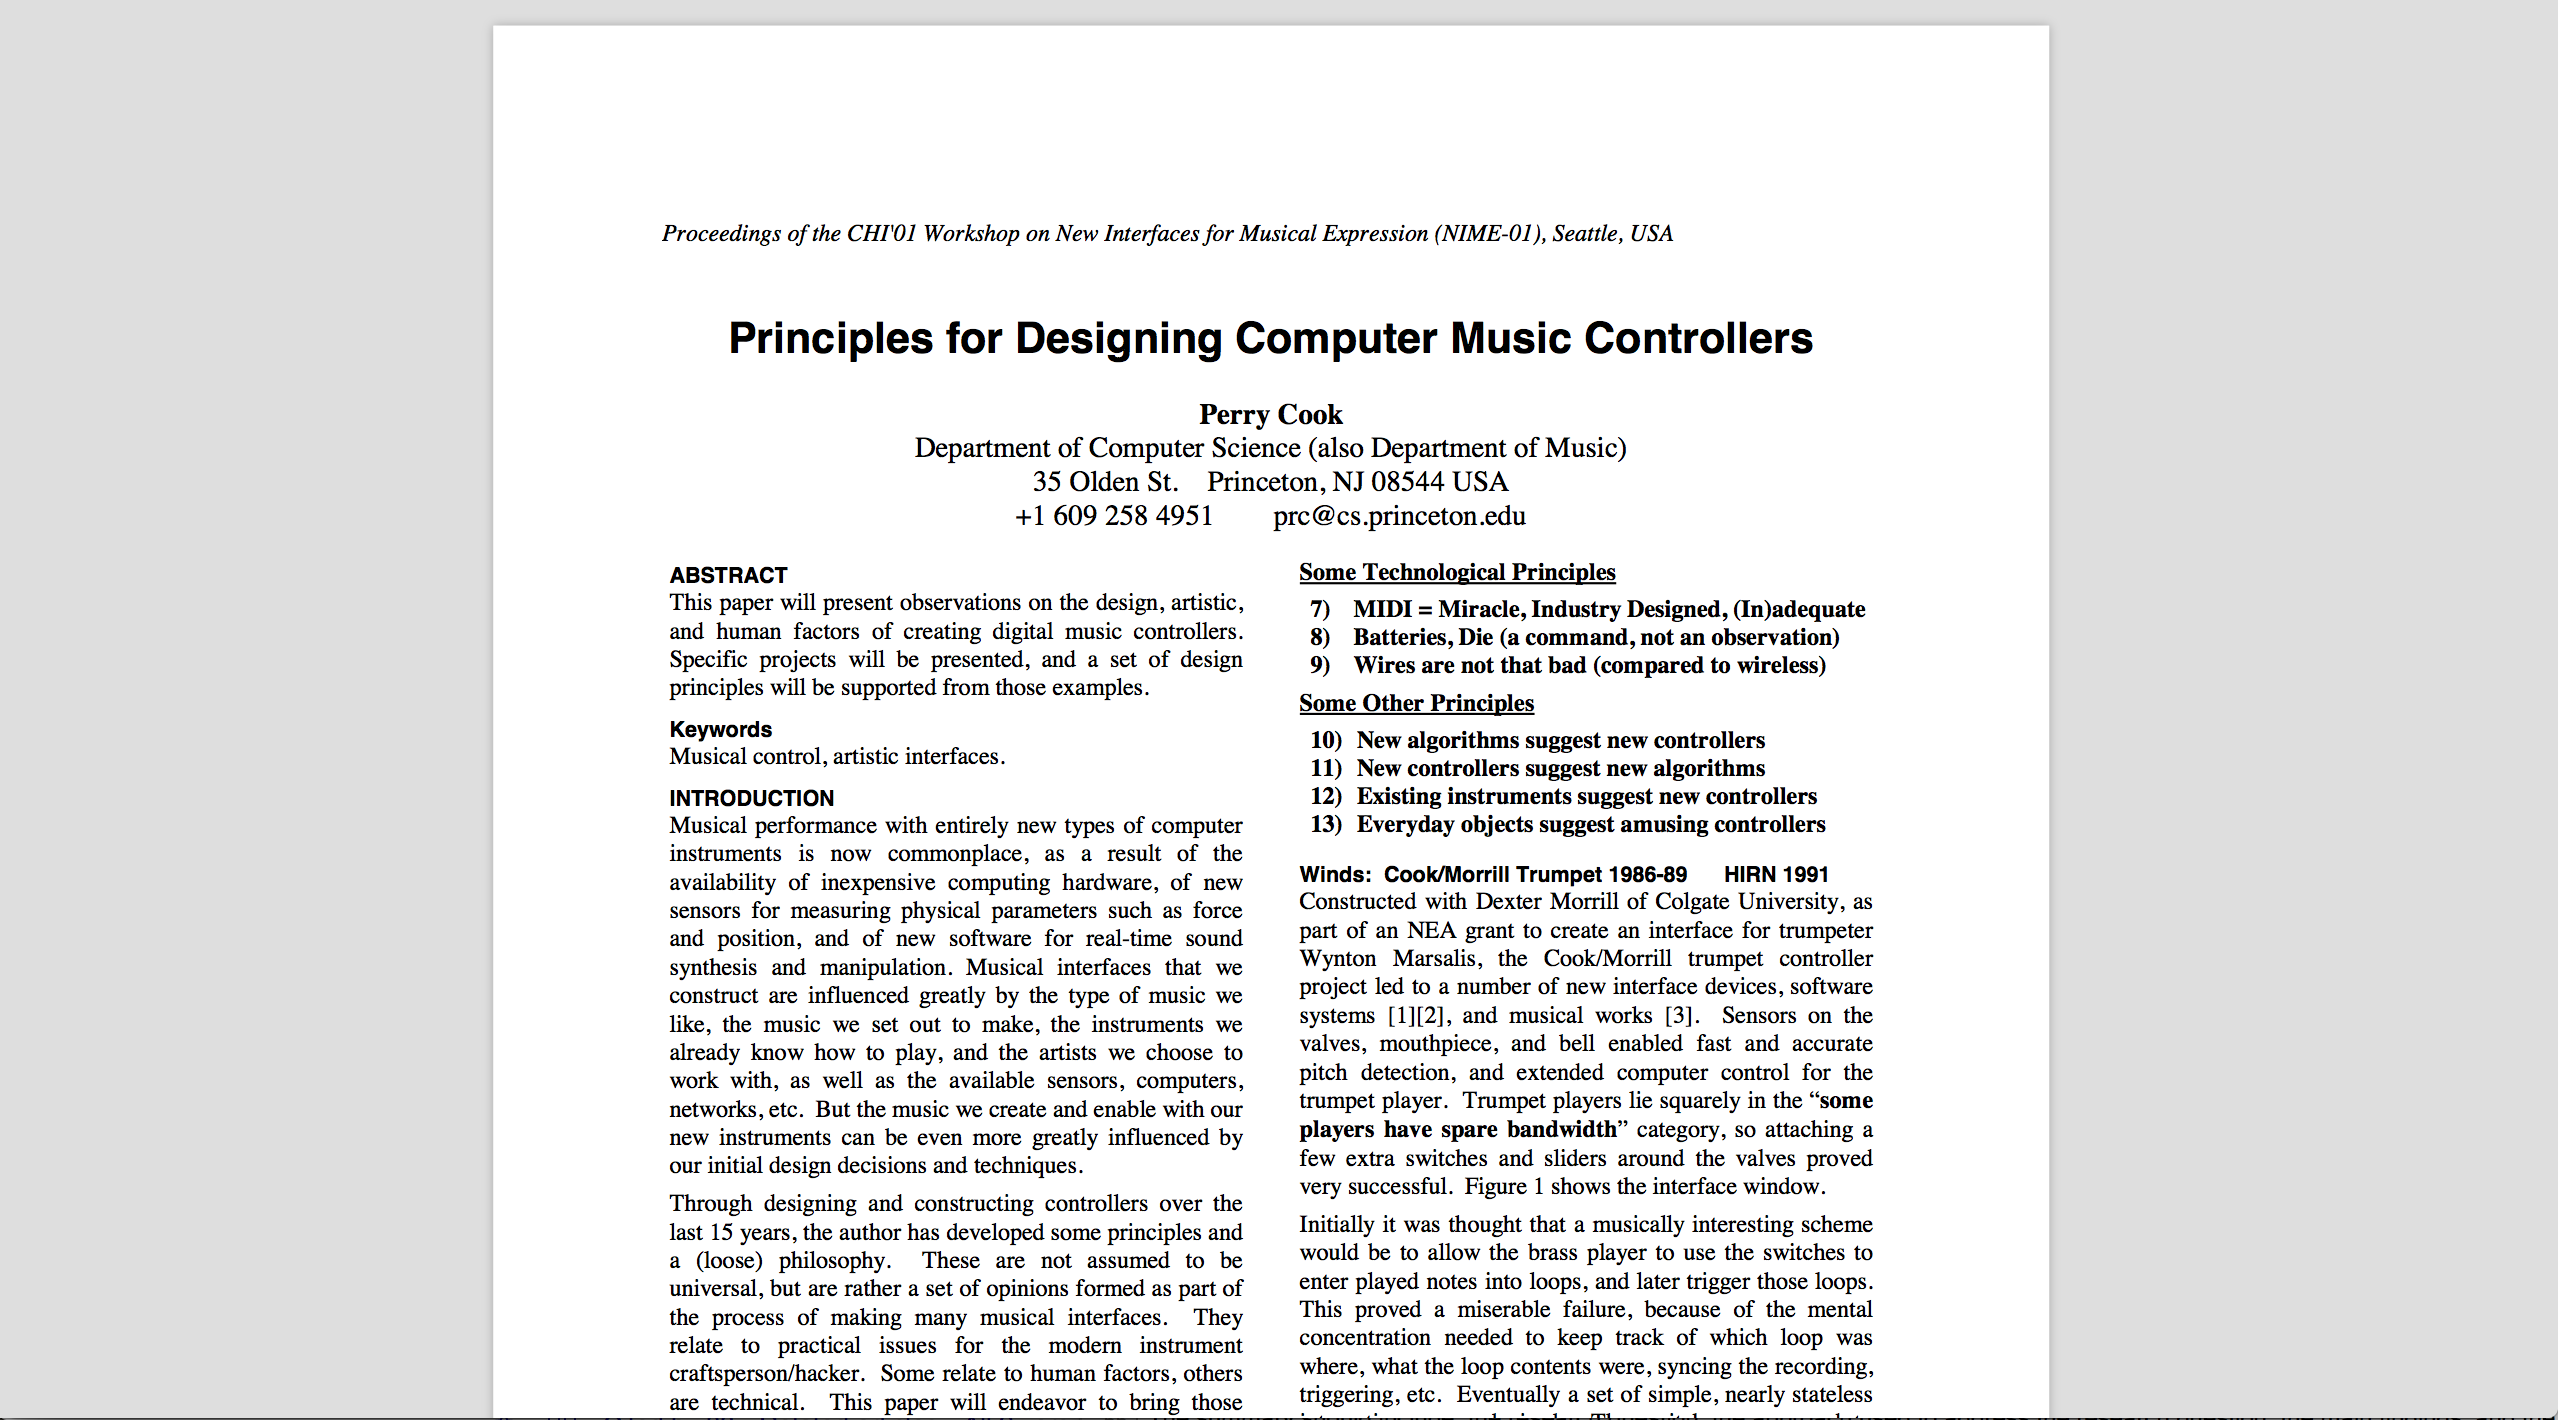
\includegraphics[scale=0.29]{img/Cook-01.png}\\
	    \cite{Cook.2001.NIME}\\
	    \url{https://www.cs.princeton.edu/~prc/CHI01Web/chi01.htm}
    \end{figure}		
\end{frame}
%
\begin{frame}
\frametitle{}
\begin{itemize}
\item Quick round: Favorite principle and why?
\item General discussion: Pros and cons of the paper?
\end{itemize}
\end{frame}
%
\begin{frame}
\frametitle{Oblique Strategies\\\small{Over One Hundred Worthwhile Dilemmas}}
\begin{figure}
	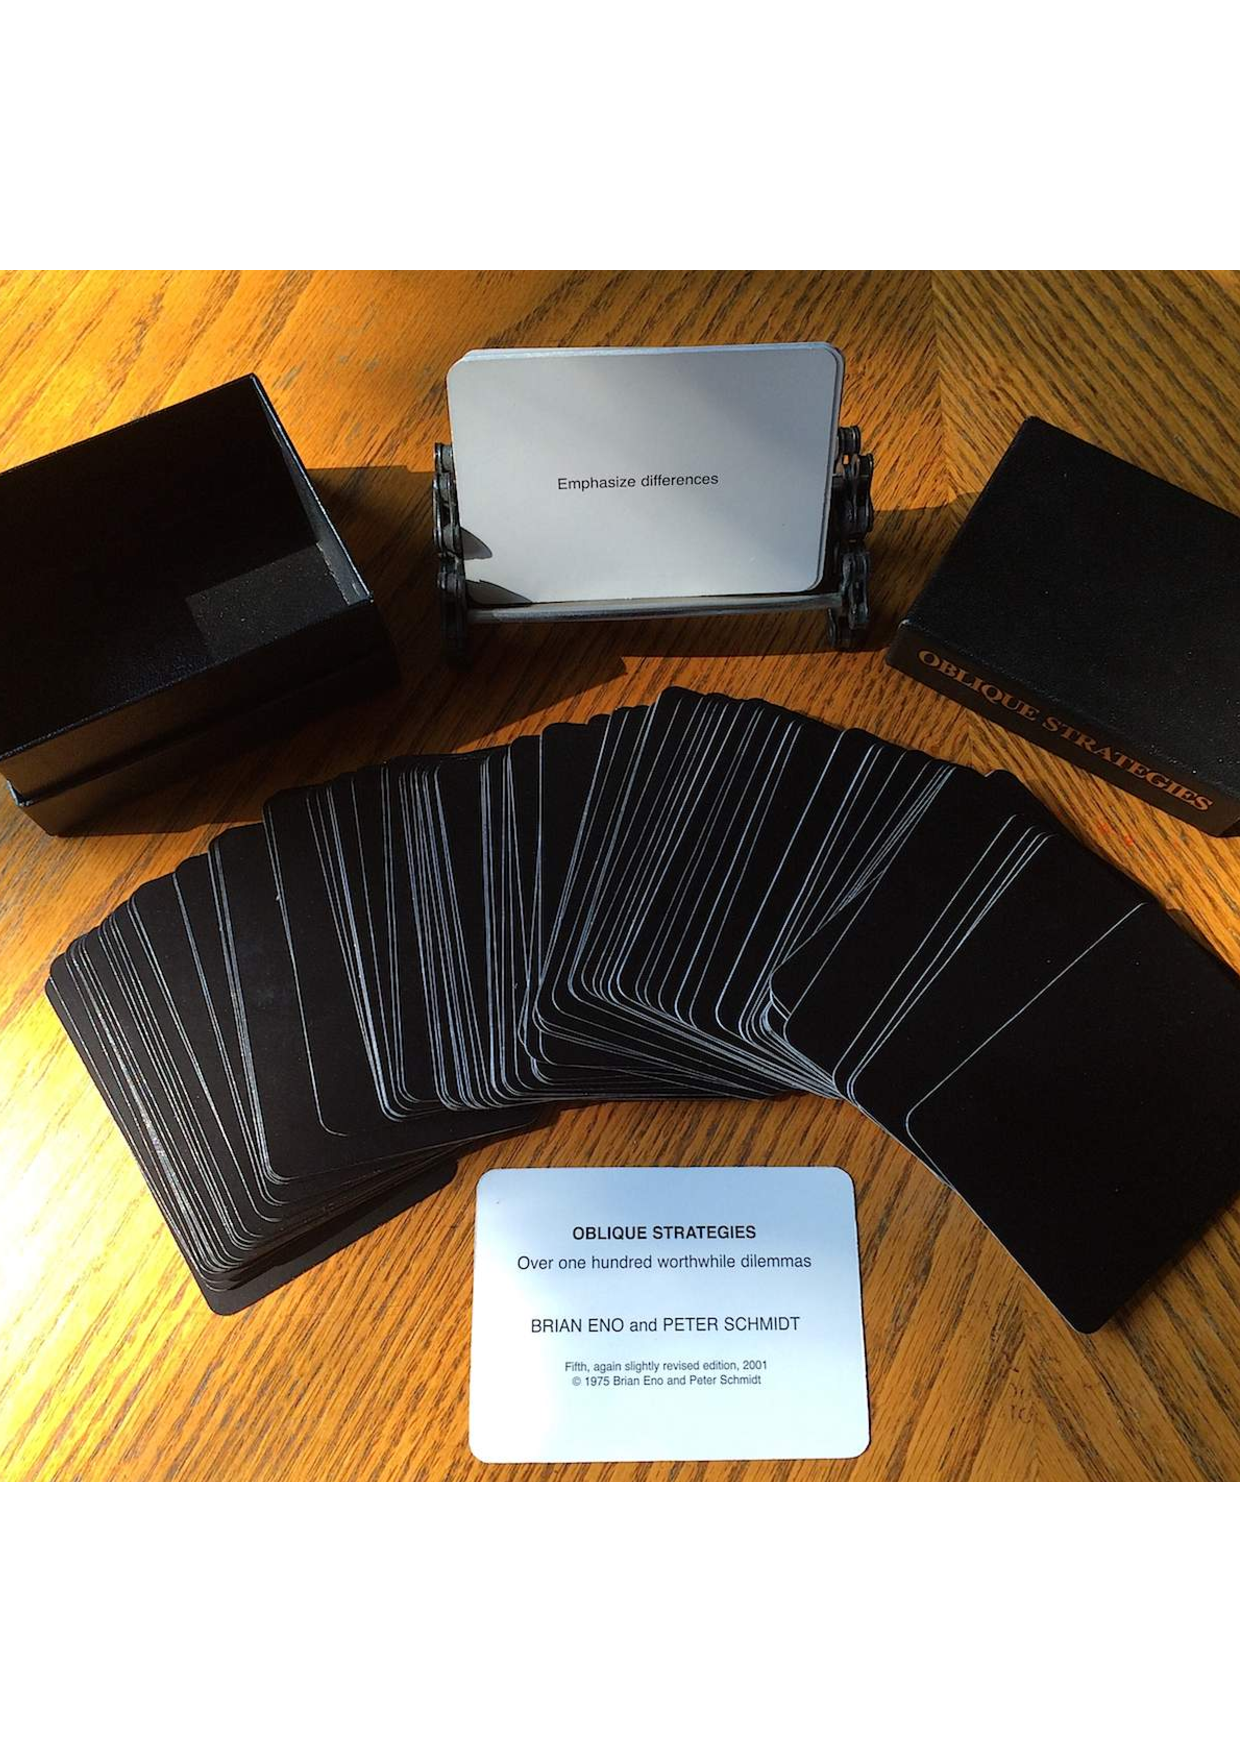
\includegraphics[scale=0.25]{img/Eno-oblique-strategies.pdf}\\
	 A card-based method for promoting creativity by Brian Eno and Peter Schmidt\\
	    \url{http://stoney.sb.org/eno/oblique.html}
    \end{figure}		
\end{frame}
%
\begin{frame}
\frametitle{Digital Lutherie}
\begin{itemize}
\item A \emph{digital luthier} is a term coined by Jord� (2005) \cite{Jorda.2005.PhD} to refer to a person who makes or remakes digital musical instruments.
\item In DMIs, there is a modular distinction between the element of control (e.g. the input device or gesture controller) and the element of sound generation. 
\item This contrasts with acoustic musical instruments, in which both elements are coupled.
\end{itemize}
\end{frame}
%
\begin{frame}
\frametitle{Digital Lutherie}
\begin{figure}
	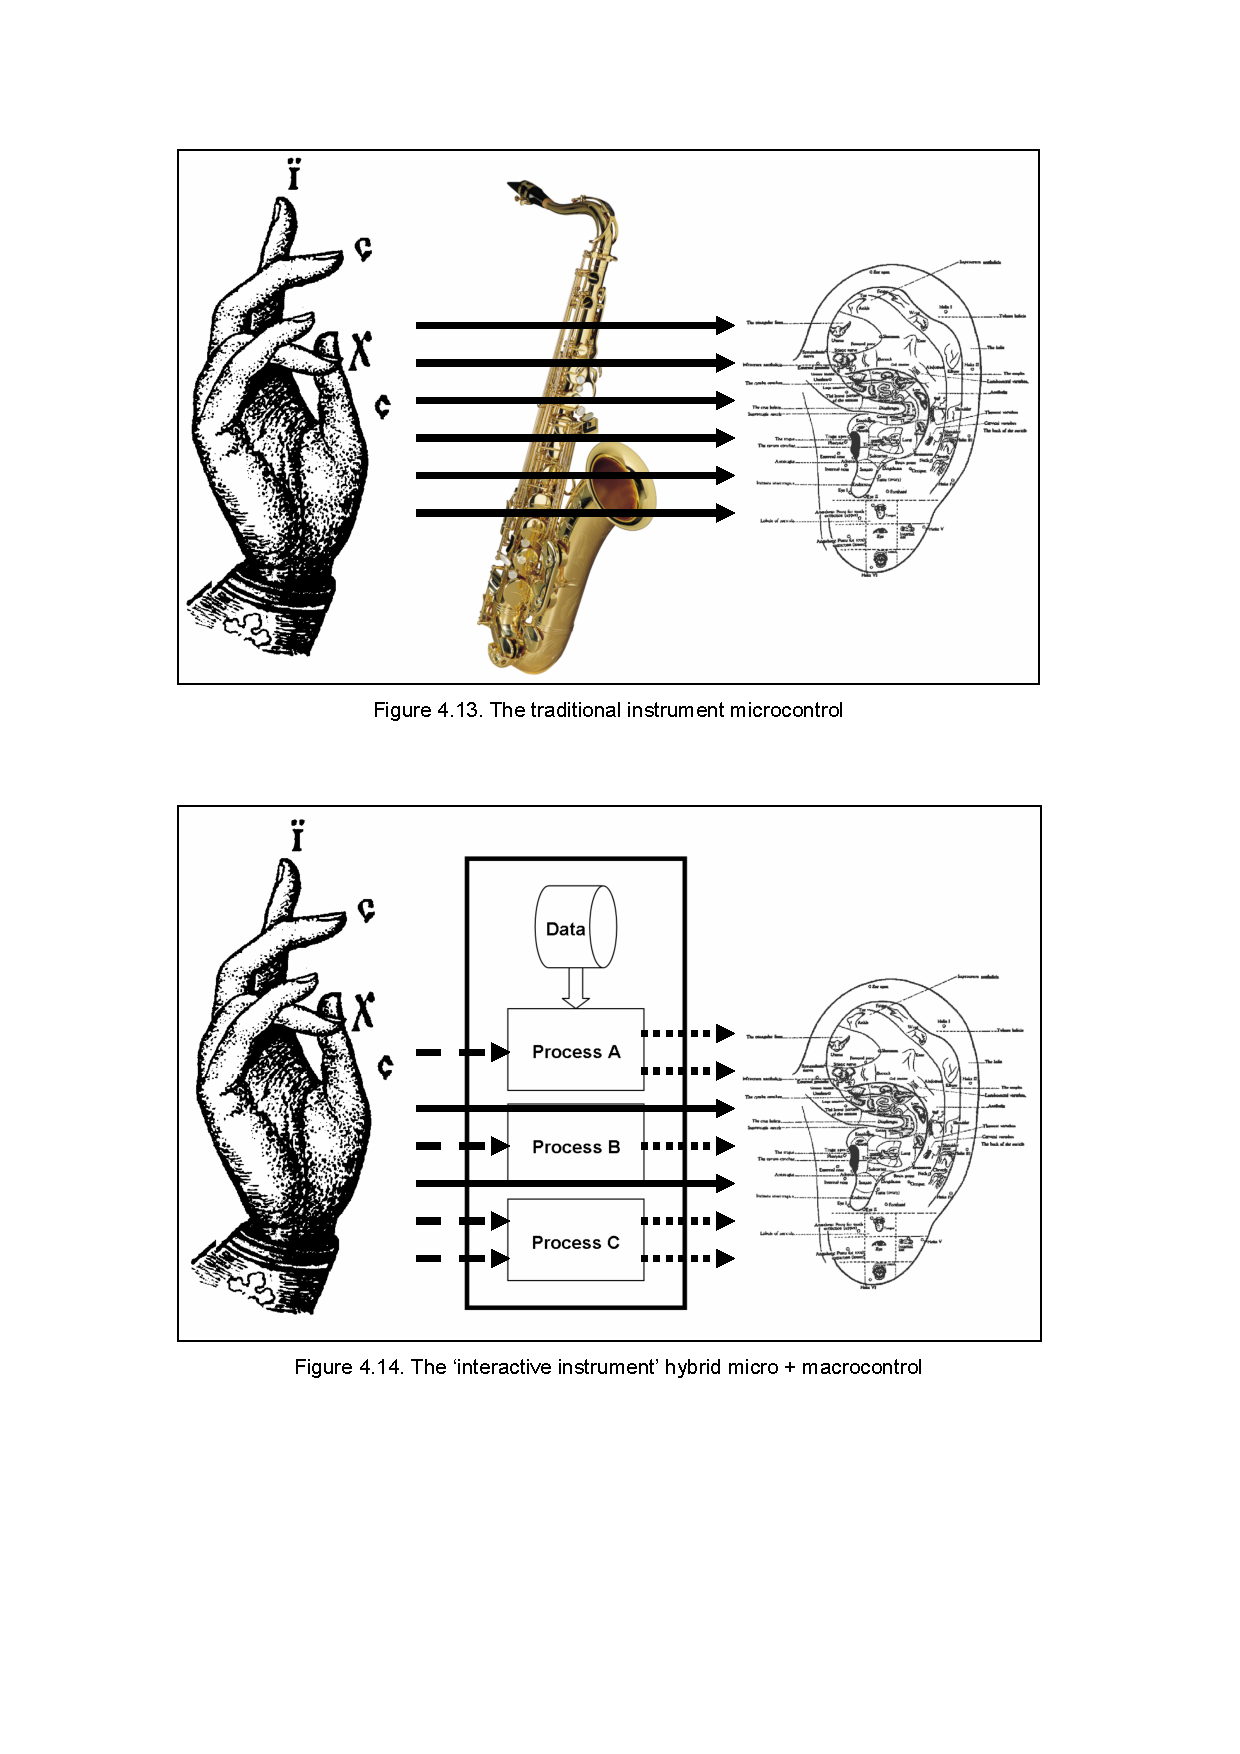
\includegraphics[scale=0.3]{img/Jorda-2005.pdf}\\
	   \cite[p.95]{Jorda.2005.PhD}
    \end{figure}		
\end{frame}
%
\begin{frame}
\frametitle{Interactive Composing Systems}
\begin{quote}
The computer responds to the performer and the performer reacts to the computer, and the music takes its form through the mutually influential, interactive relationship. Joel Chadabe, 1984 \cite[p.23]{Chadabe.1984.CMJ}
\end{quote}
\end{frame}
%
\begin{frame}
\frametitle{Interactive Composing Systems}
\begin{figure}
	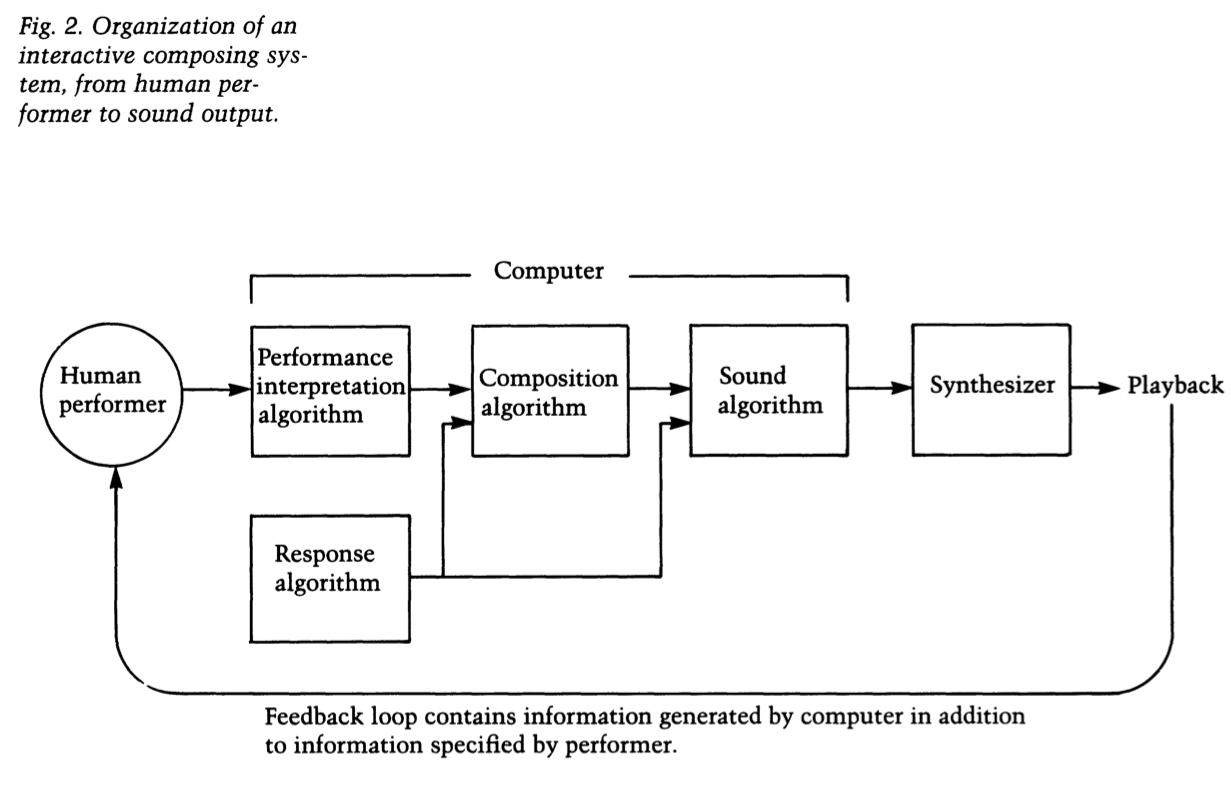
\includegraphics[scale=0.45]{img/Chadabe-1984.png}\\
	    \cite[p.24]{Chadabe.1984.CMJ}
    \end{figure}		
\end{frame}
%
\begin{frame}
\frametitle{}
\begin{figure}
	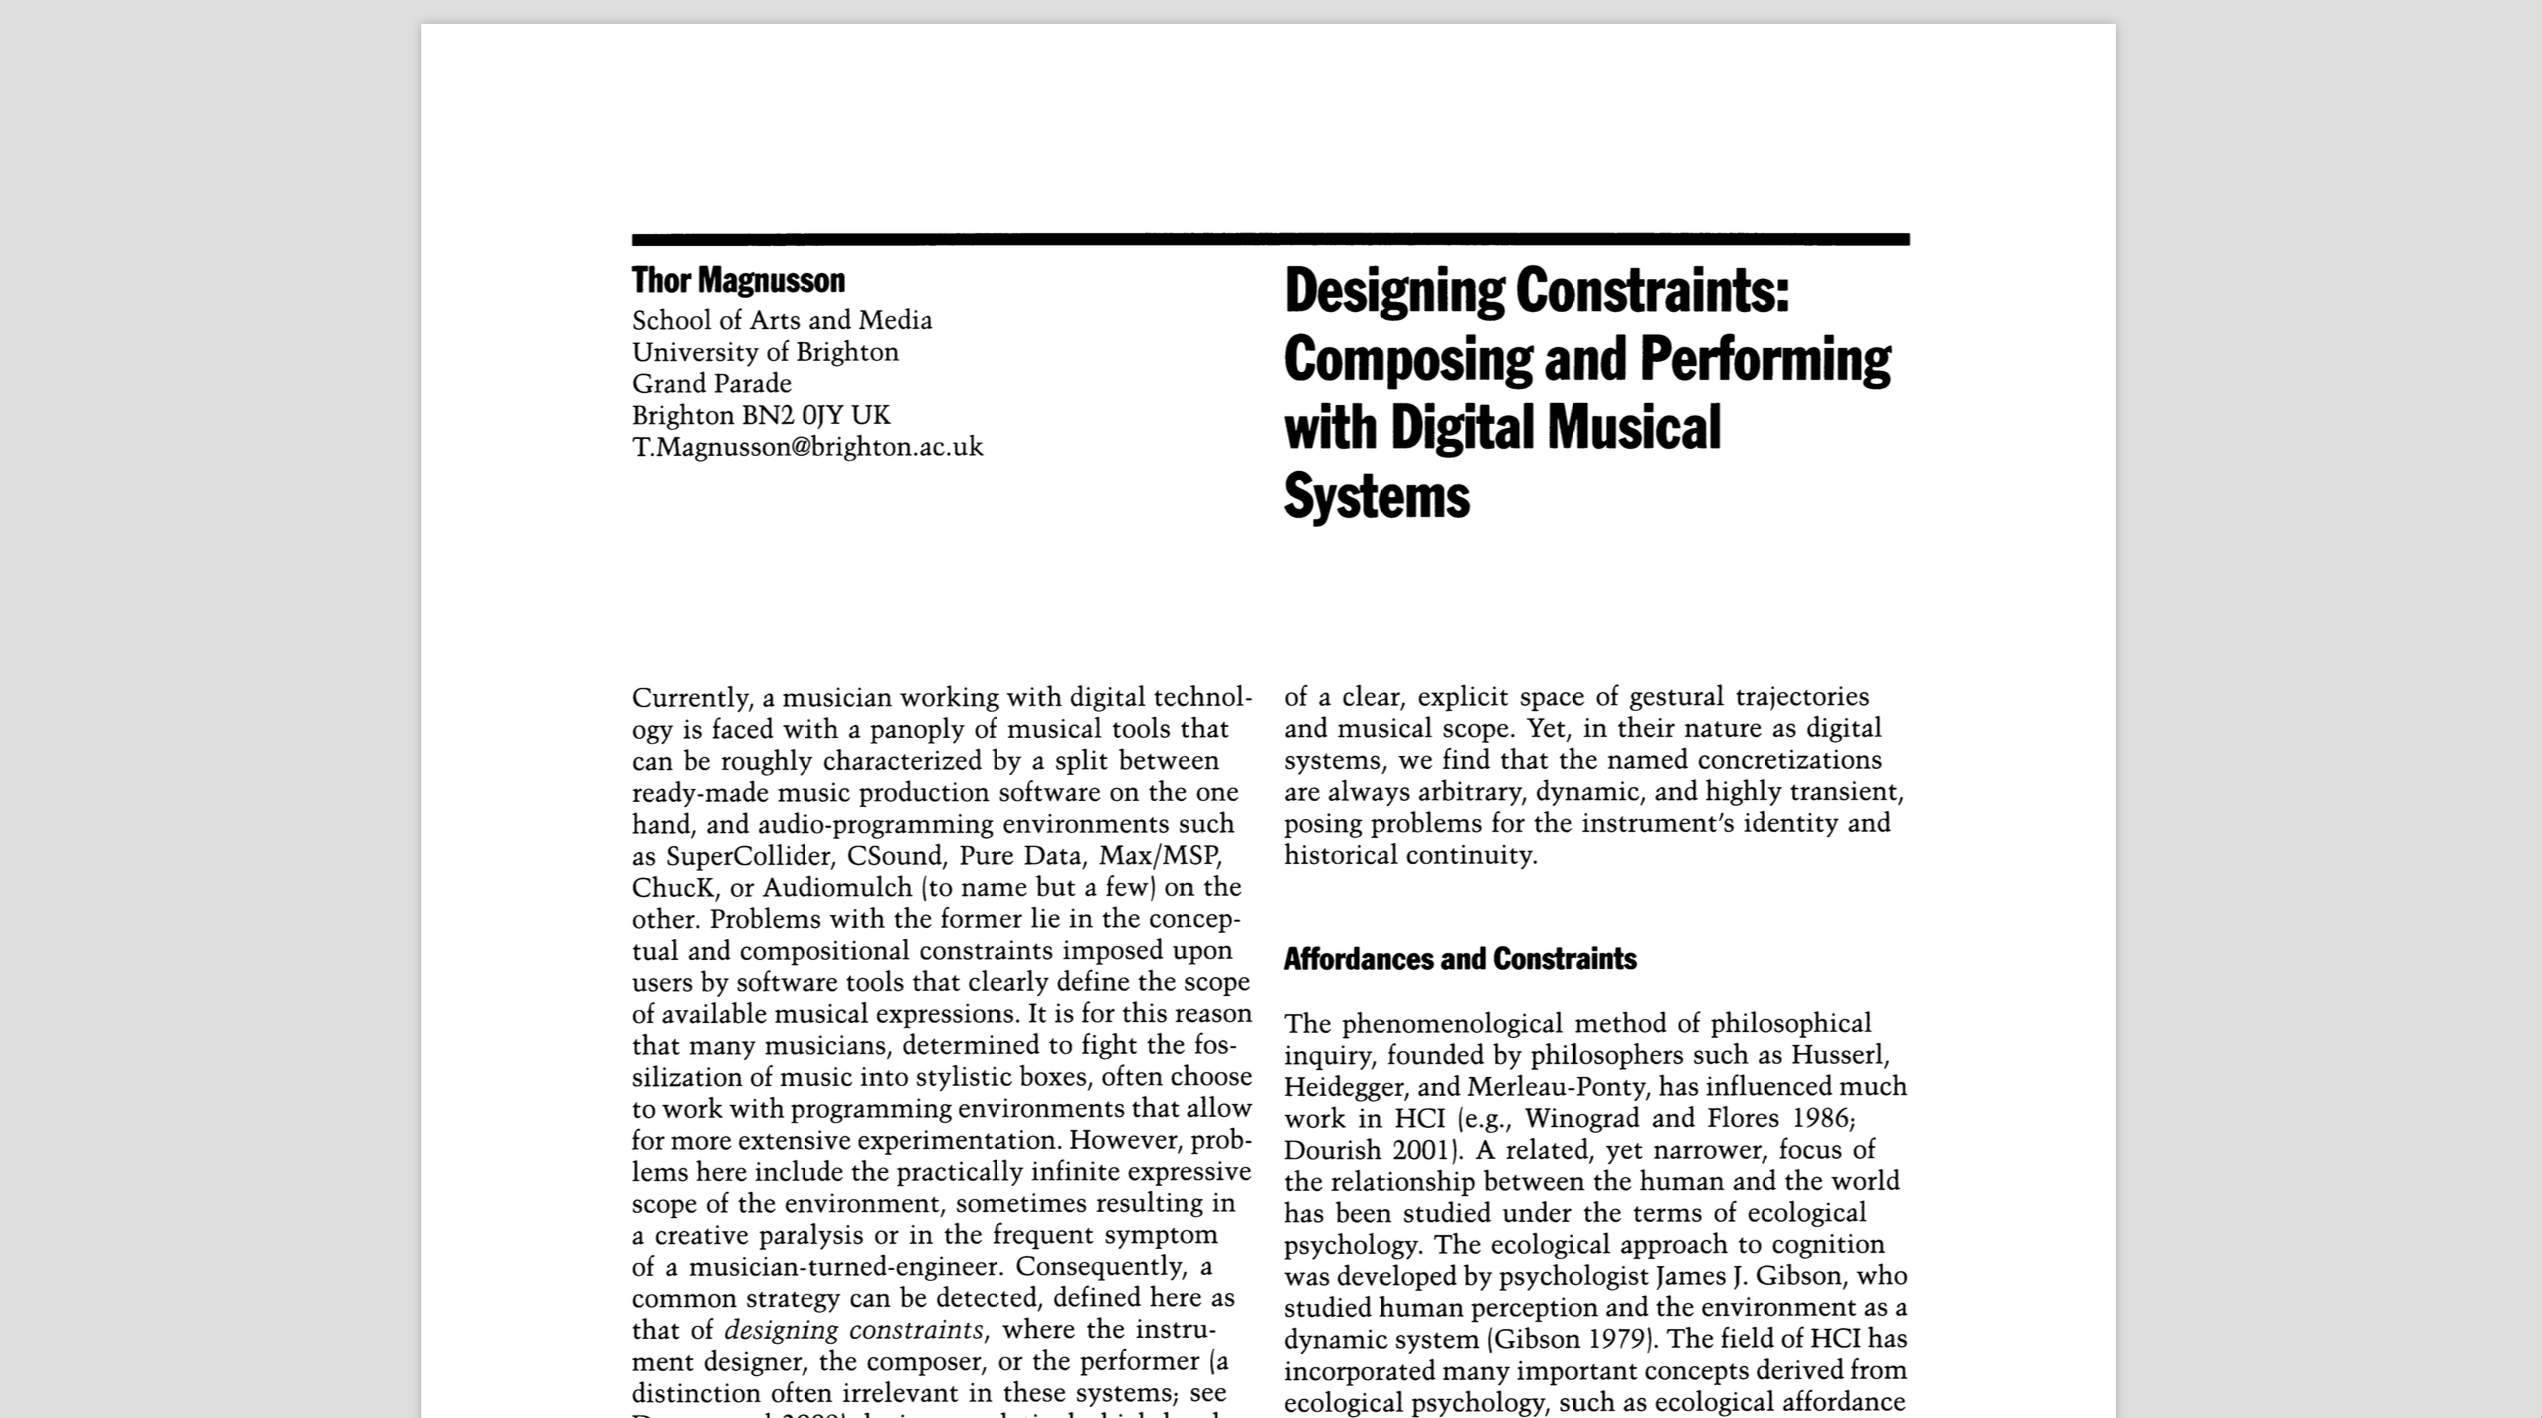
\includegraphics[scale=0.3]{img/Magnusson-2010.png}\\
	    \cite{Magnusson.2010.constraints}
    \end{figure}		
\end{frame}
%
\begin{frame}
\frametitle{Designing Constraints}
\begin{itemize}
\item HCI concepts: \emph{Affordances}, \emph{constraints} and \emph{mapping}.
\item Perceived \emph{affordances}: the properties that the agent perceives as possible actions upon an object (Norman 1988).
\item \emph{Constraints} map out a territory of structural possibilities which can then be explored, and perhaps transformed to give another one (Boden 1990, p. 95).
\item \emph{Mapping} as designing constraints: the sound and mapping engines serve as the core of the digital musical instrument, they are its ``real body''.
\end{itemize}	
\end{frame}
%
\begin{frame}
\frametitle{Designing Constraints}
\begin{itemize}
\item Mapping should be defined as a compositional process that engenders a structure of constraints.
\item Design of constraints, where the making of the instrument involves composition, or alternatively, composing involves instrument design.
\item The primary character of a new NIME is defined by its constraints (affordances are provided by the hardware and software features).
\item Affordances point to features that make things possible and constraints define the limits of the possible.
\end{itemize}	
\end{frame}
%
\begin{frame}
\frametitle{Designing Constraints}
\begin{figure}
	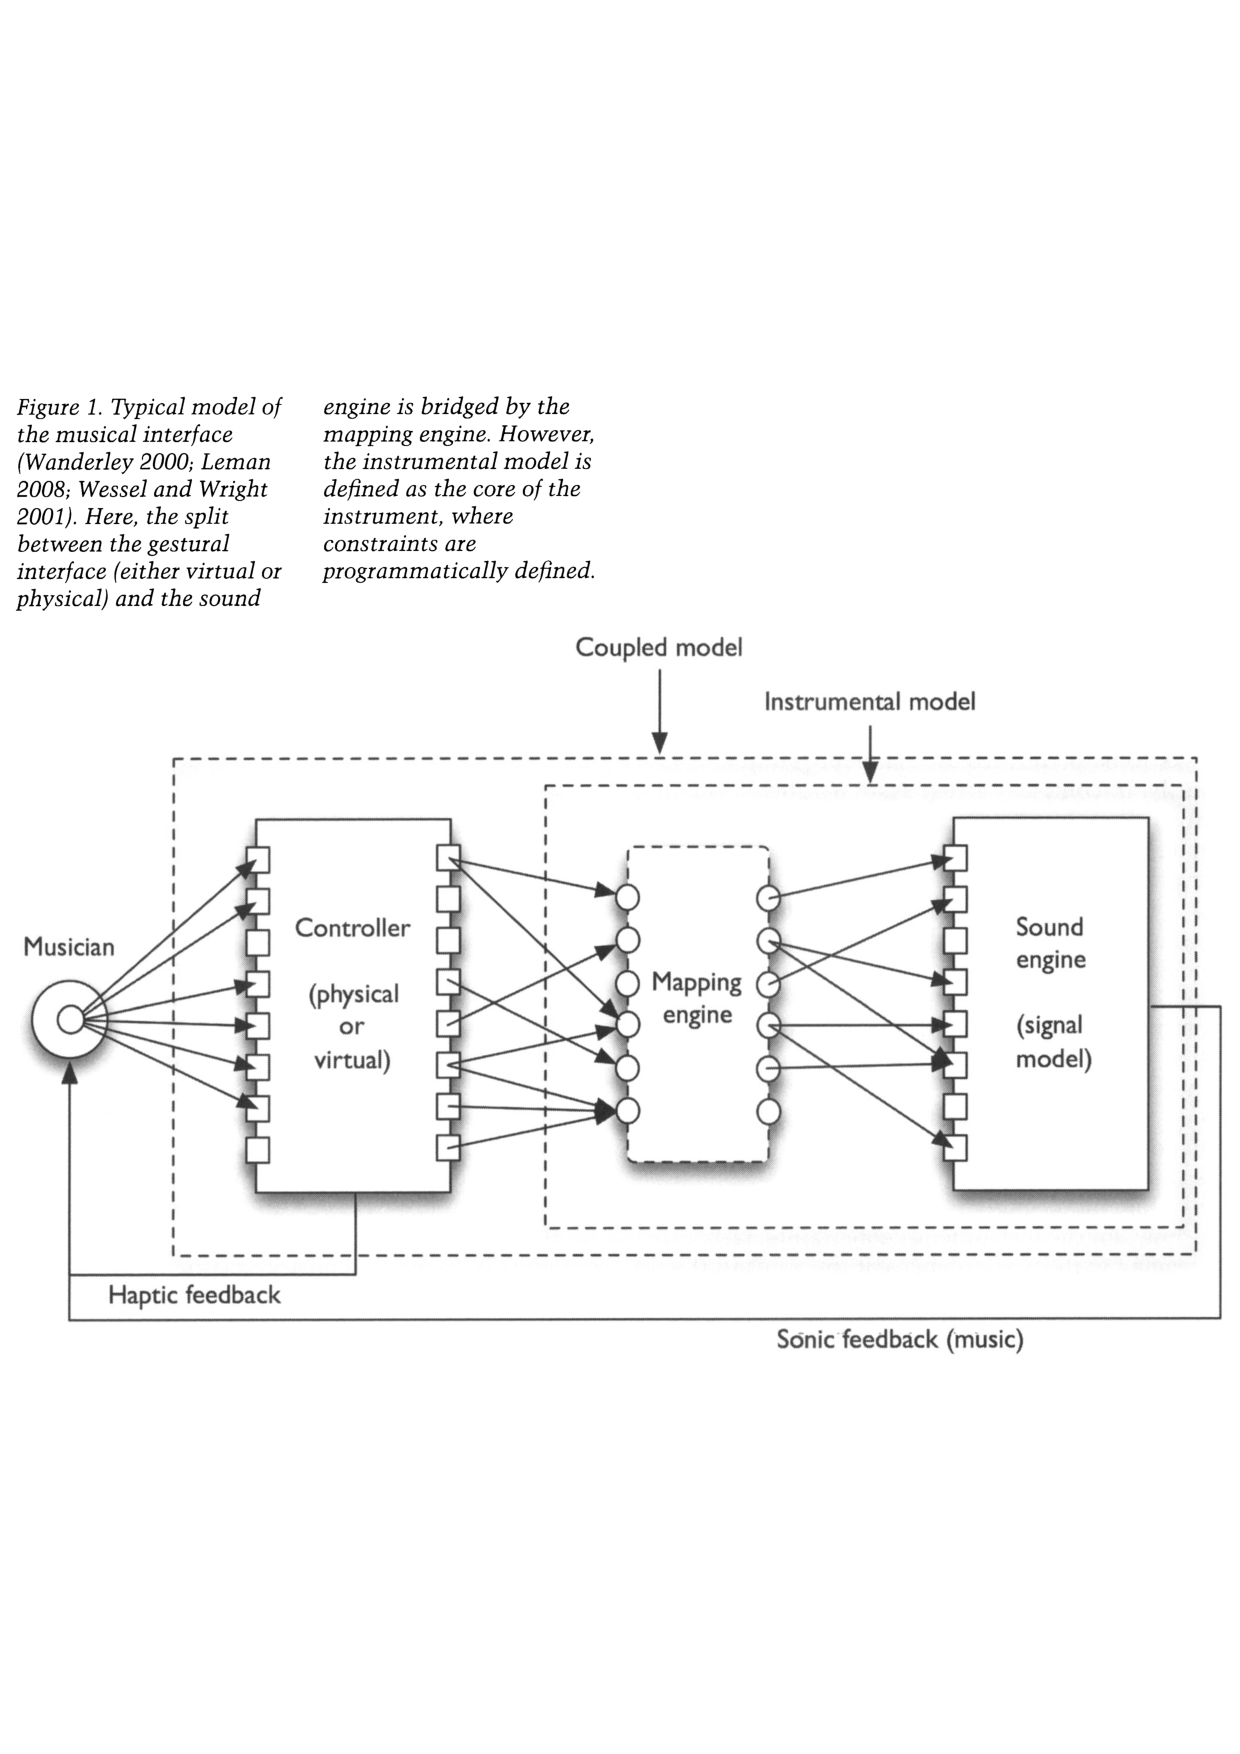
\includegraphics[scale=0.38]{img/Magnusson-2010-mappings.pdf}\\
	    \cite[p.66]{Magnusson.2010.constraints}
    \end{figure}		
\end{frame}
%
\begin{frame}
\frametitle{}
\begin{figure}
	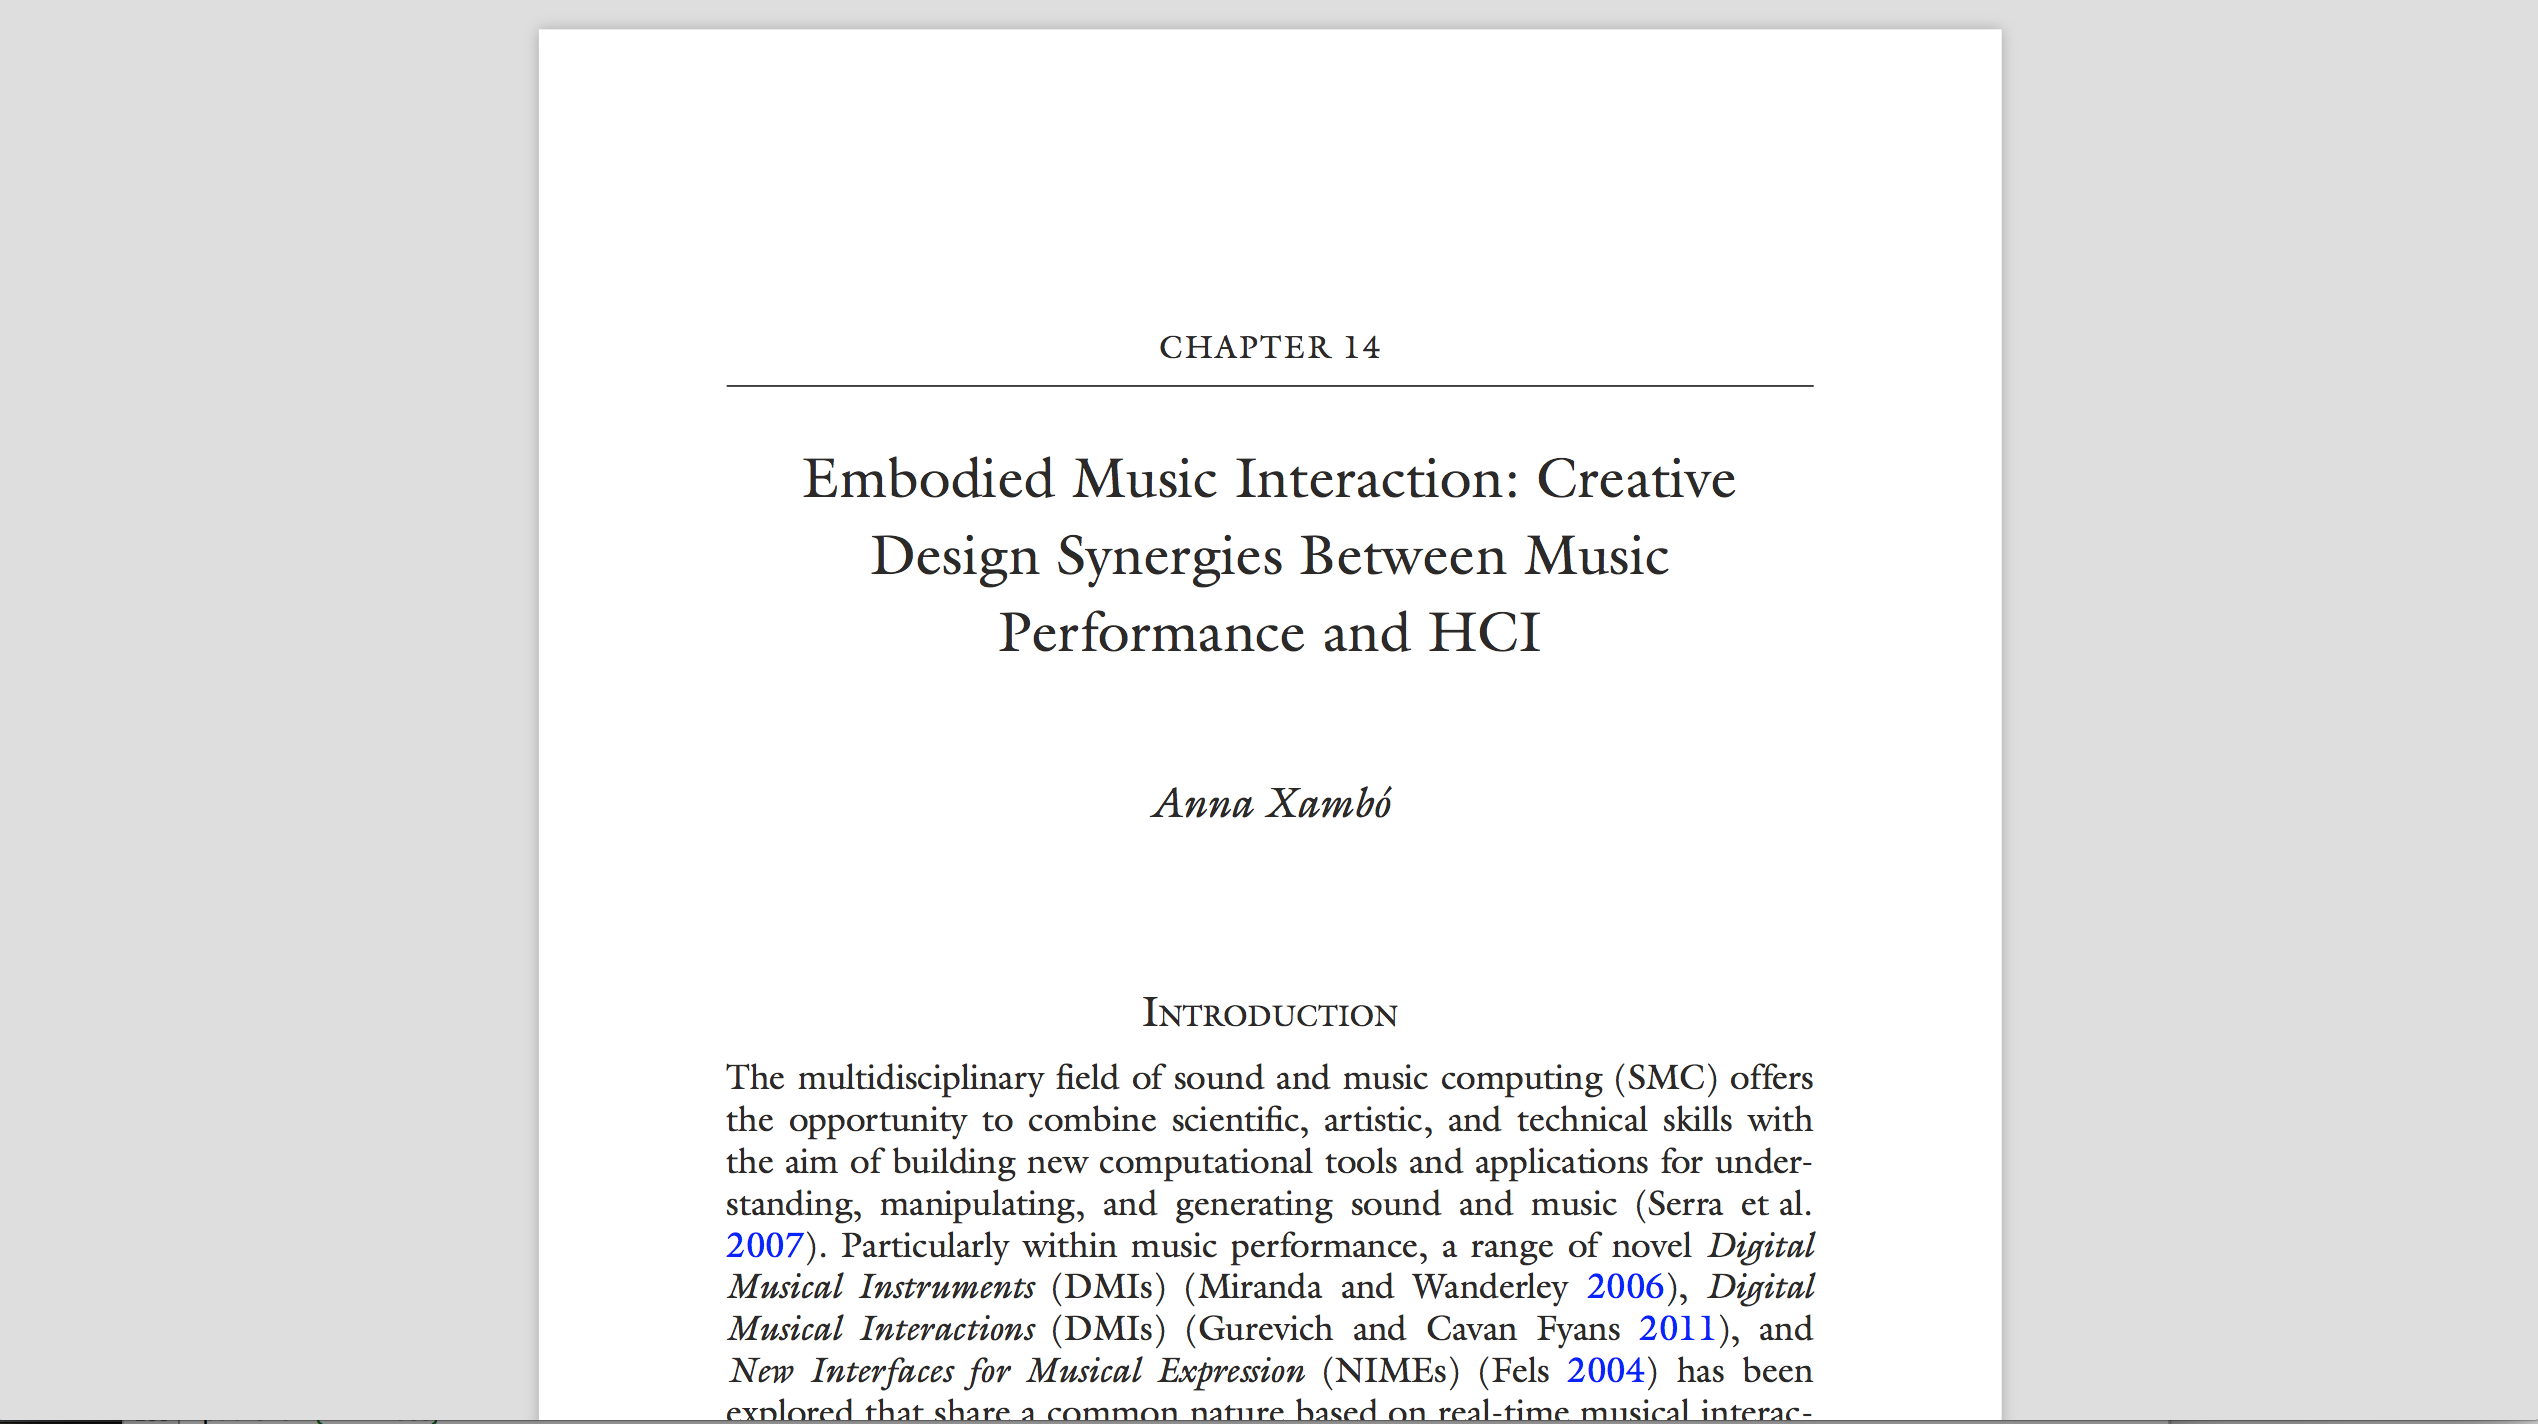
\includegraphics[scale=0.3]{img/Xambo-2017.png}\\
	    \cite{Xambo.2017.EMI}
    \end{figure}		
\end{frame}
%
\begin{frame}
\frametitle{Embodied Music Interaction}
\begin{itemize}
\item We can adapt the HCI theoretical framework of embodied interaction with the aim of informing the design of DMIs.
\item Meaning is co-constructed through making within a social context and is mediated by the technology used (Dourish (2001) \cite{Dourish.2004.embodiedinteraction}).
\item Embodied interaction involves considering the role of the \emph{body}, the \emph{social world}, and the \emph{physical world}, all three within a \emph{situated context} (for \emph{situated action} see Suchman (1987) \cite{Suchman.1987.situatedaction}).
\item Embodied interaction involves designing interfaces that require complex bodily interactions.
\end{itemize}	
\end{frame}
%
\begin{frame}
\frametitle{Embodied Music Interaction}
\begin{quote}
A piece of jewelry is in a sense an object that is not complete in itself. Jewelry is a `what is it?' until you relate it to the body. The body is a component in design just as air and space are. Like line, form, and color, the body is a material to work with. It is one of the basic inspirations in creating form. (Art Smith 1969)
\end{quote}
Embodied Music Interaction: one can say that the body is an important aspect in music technology design, just like melody, harmony, rhythm, dynamics, and timbre.
\end{frame}
%
\begin{frame}
\frametitle{Embodied Music Interaction}
\begin{itemize}
\item \emph{Embodied music interaction} challenges and potentials of embodied interaction using DMIs for music performance.
\item The consideration of embodied interaction in DMI design can improve rethinking of the: 
\begin{enumerate}
\item communication with the audience, and performers; 
\item the shareability and collaborative features, allowing for scalability of the system; and 
\item the materiality and space features, including connections between digital and physical spaces in the interface, and the space between and outside the practitioner and the musical instrument.
\end{enumerate}
\end{itemize}	
\end{frame}
%
\begin{frame}
\frametitle{Embodied Music Interaction}
\begin{figure}
	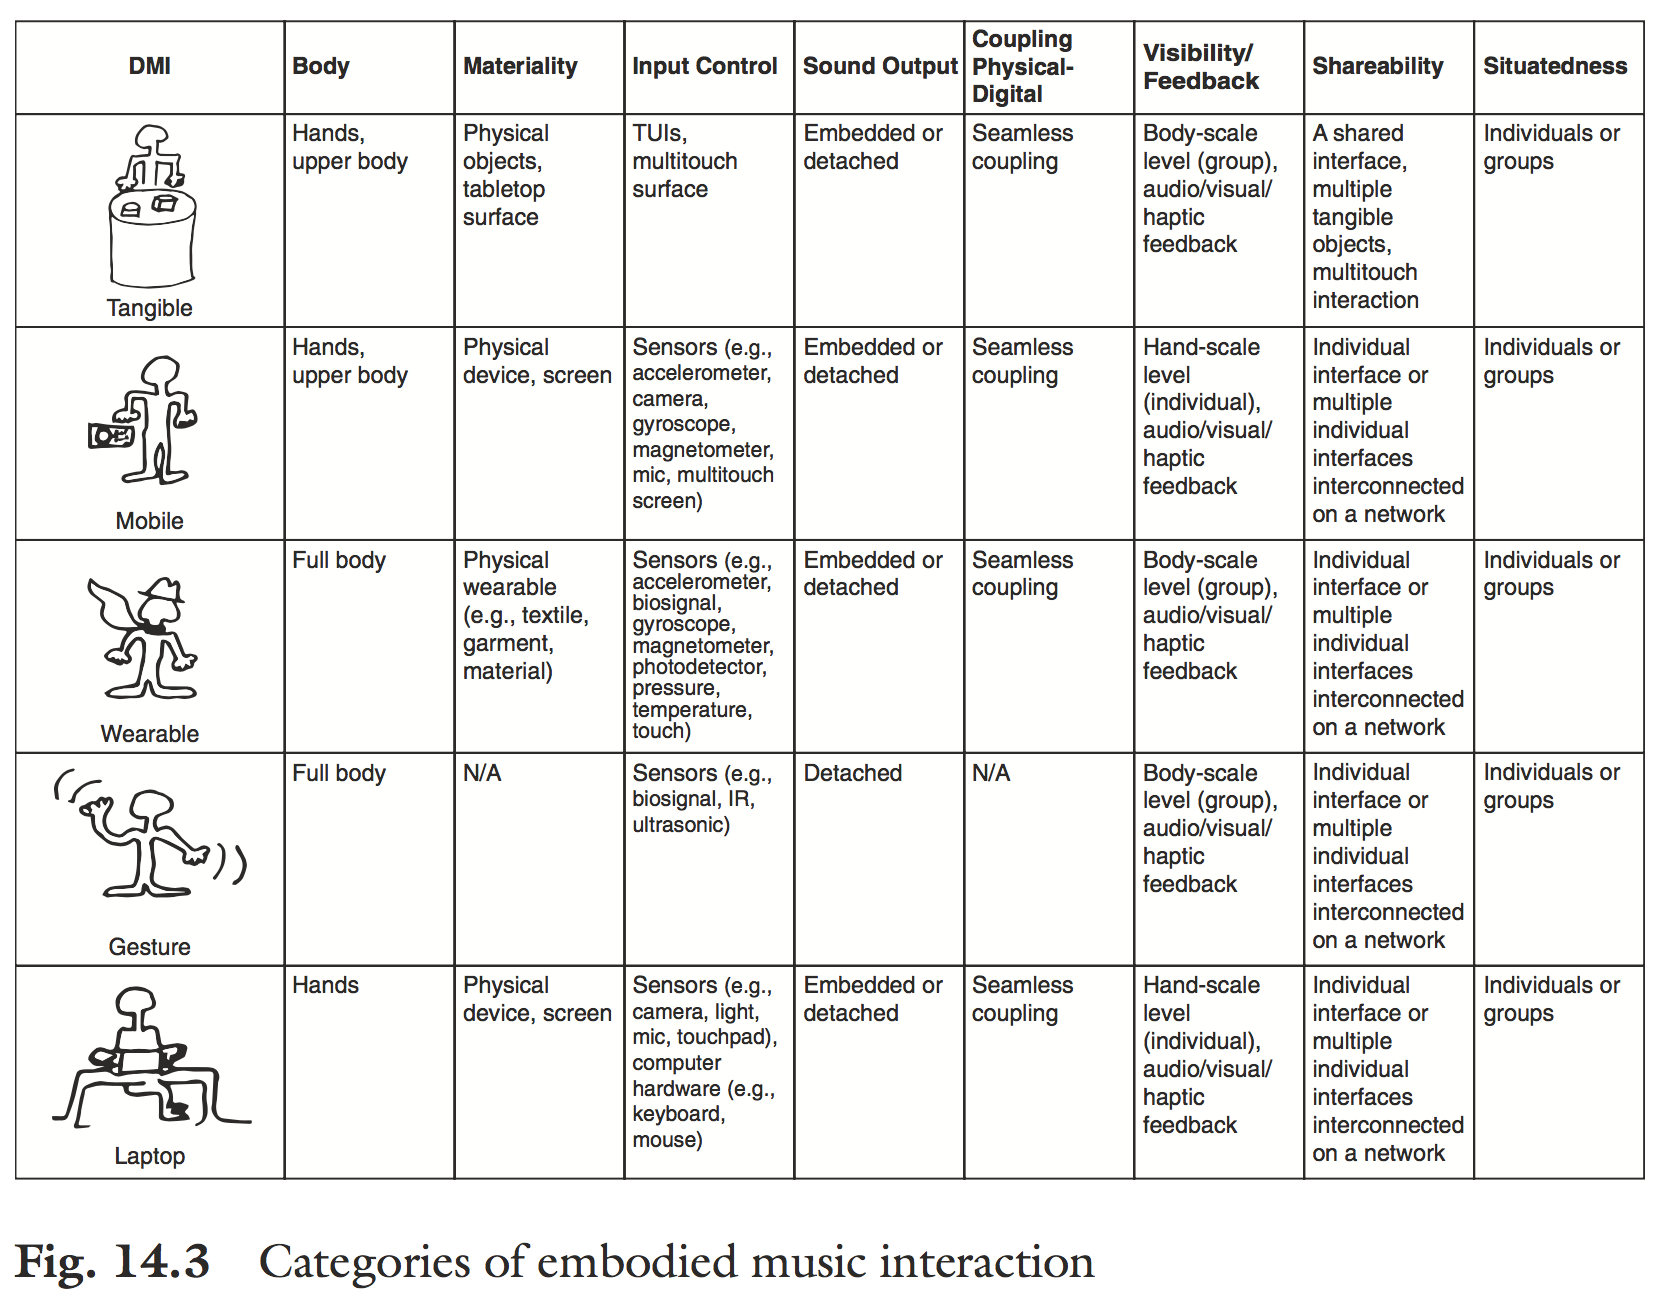
\includegraphics[scale=0.28]{img/Xambo-2017-categories-EMI.png}\\
	    \cite[p.213]{Xambo.2017.EMI}
    \end{figure}		
\end{frame}
%
\begin{frame}
\frametitle{}
\Huge{Representing and documenting NIMEs}
\end{frame}
%
\begin{frame}
\frametitle{Videos}
\begin{itemize}
\item Bill Buxton's SSSP
\begin{itemize}
	\item SSSP Overview: \\
	\url{https://www.youtube.com/watch?v=4DiREhbB6Nw}
	\item The SSSP Interactive Performance System: \url{https://www.youtube.com/watch?v=cHmf36J-EEE}
\end{itemize}
\item Bill Buxton videos: \url{https://www.billbuxton.com/buxtonVideos.html}
\item Reactable basic demo \#1: \url{https://www.youtube.com/watch?v=0h-RhyopUmc}
\end{itemize}
\end{frame}
%
\begin{frame}
\frametitle{Graphical Representations}
\begin{itemize}
\item Photos
\item Illustrations
\item Diagrams (see Unified Modeling Language (UML) e.g. behavioural diagrams, structural diagrams, and so on)
\item Mindmaps :)
\item and many more...
\end{itemize}
\end{frame}
%
\begin{frame}
\frametitle{Teamwork: Classification and representation of NIMEs}
\begin{itemize}
\item Take the same paper that you selected from the NIME Reader (\url{https://www.springer.com/gp/book/9783319472133}) where a NIME is presented. 
Discussion about ... 
\begin{itemize}
\item how is the instrument design presented in the paper: diagrams? photographs? mindmaps?
\item how is the NIME documented? are there videos? what are the characteristics of the documentation in particular the videos?
\end{itemize}
\end{itemize}
\end{frame}
%
\begin{frame}
\frametitle{Teamwork: Summaries}
\begin{itemize}
\item The teams summarize to the group their selected paper / NIME (5-7 minutes per group). 
\begin{itemize}
\item how is the instrument design presented in the paper: diagrams? photographs? mindmaps?
\item how is the NIME documented? are there videos? what are the characteristics of the documentation in particular the videos?
\end{itemize}
\end{itemize}
\end{frame}
%
\begin{frame}
\frametitle{}
\Huge{And now all begins...}
\end{frame}
%
\begin{frame}
\frametitle{}
\begin{figure}
	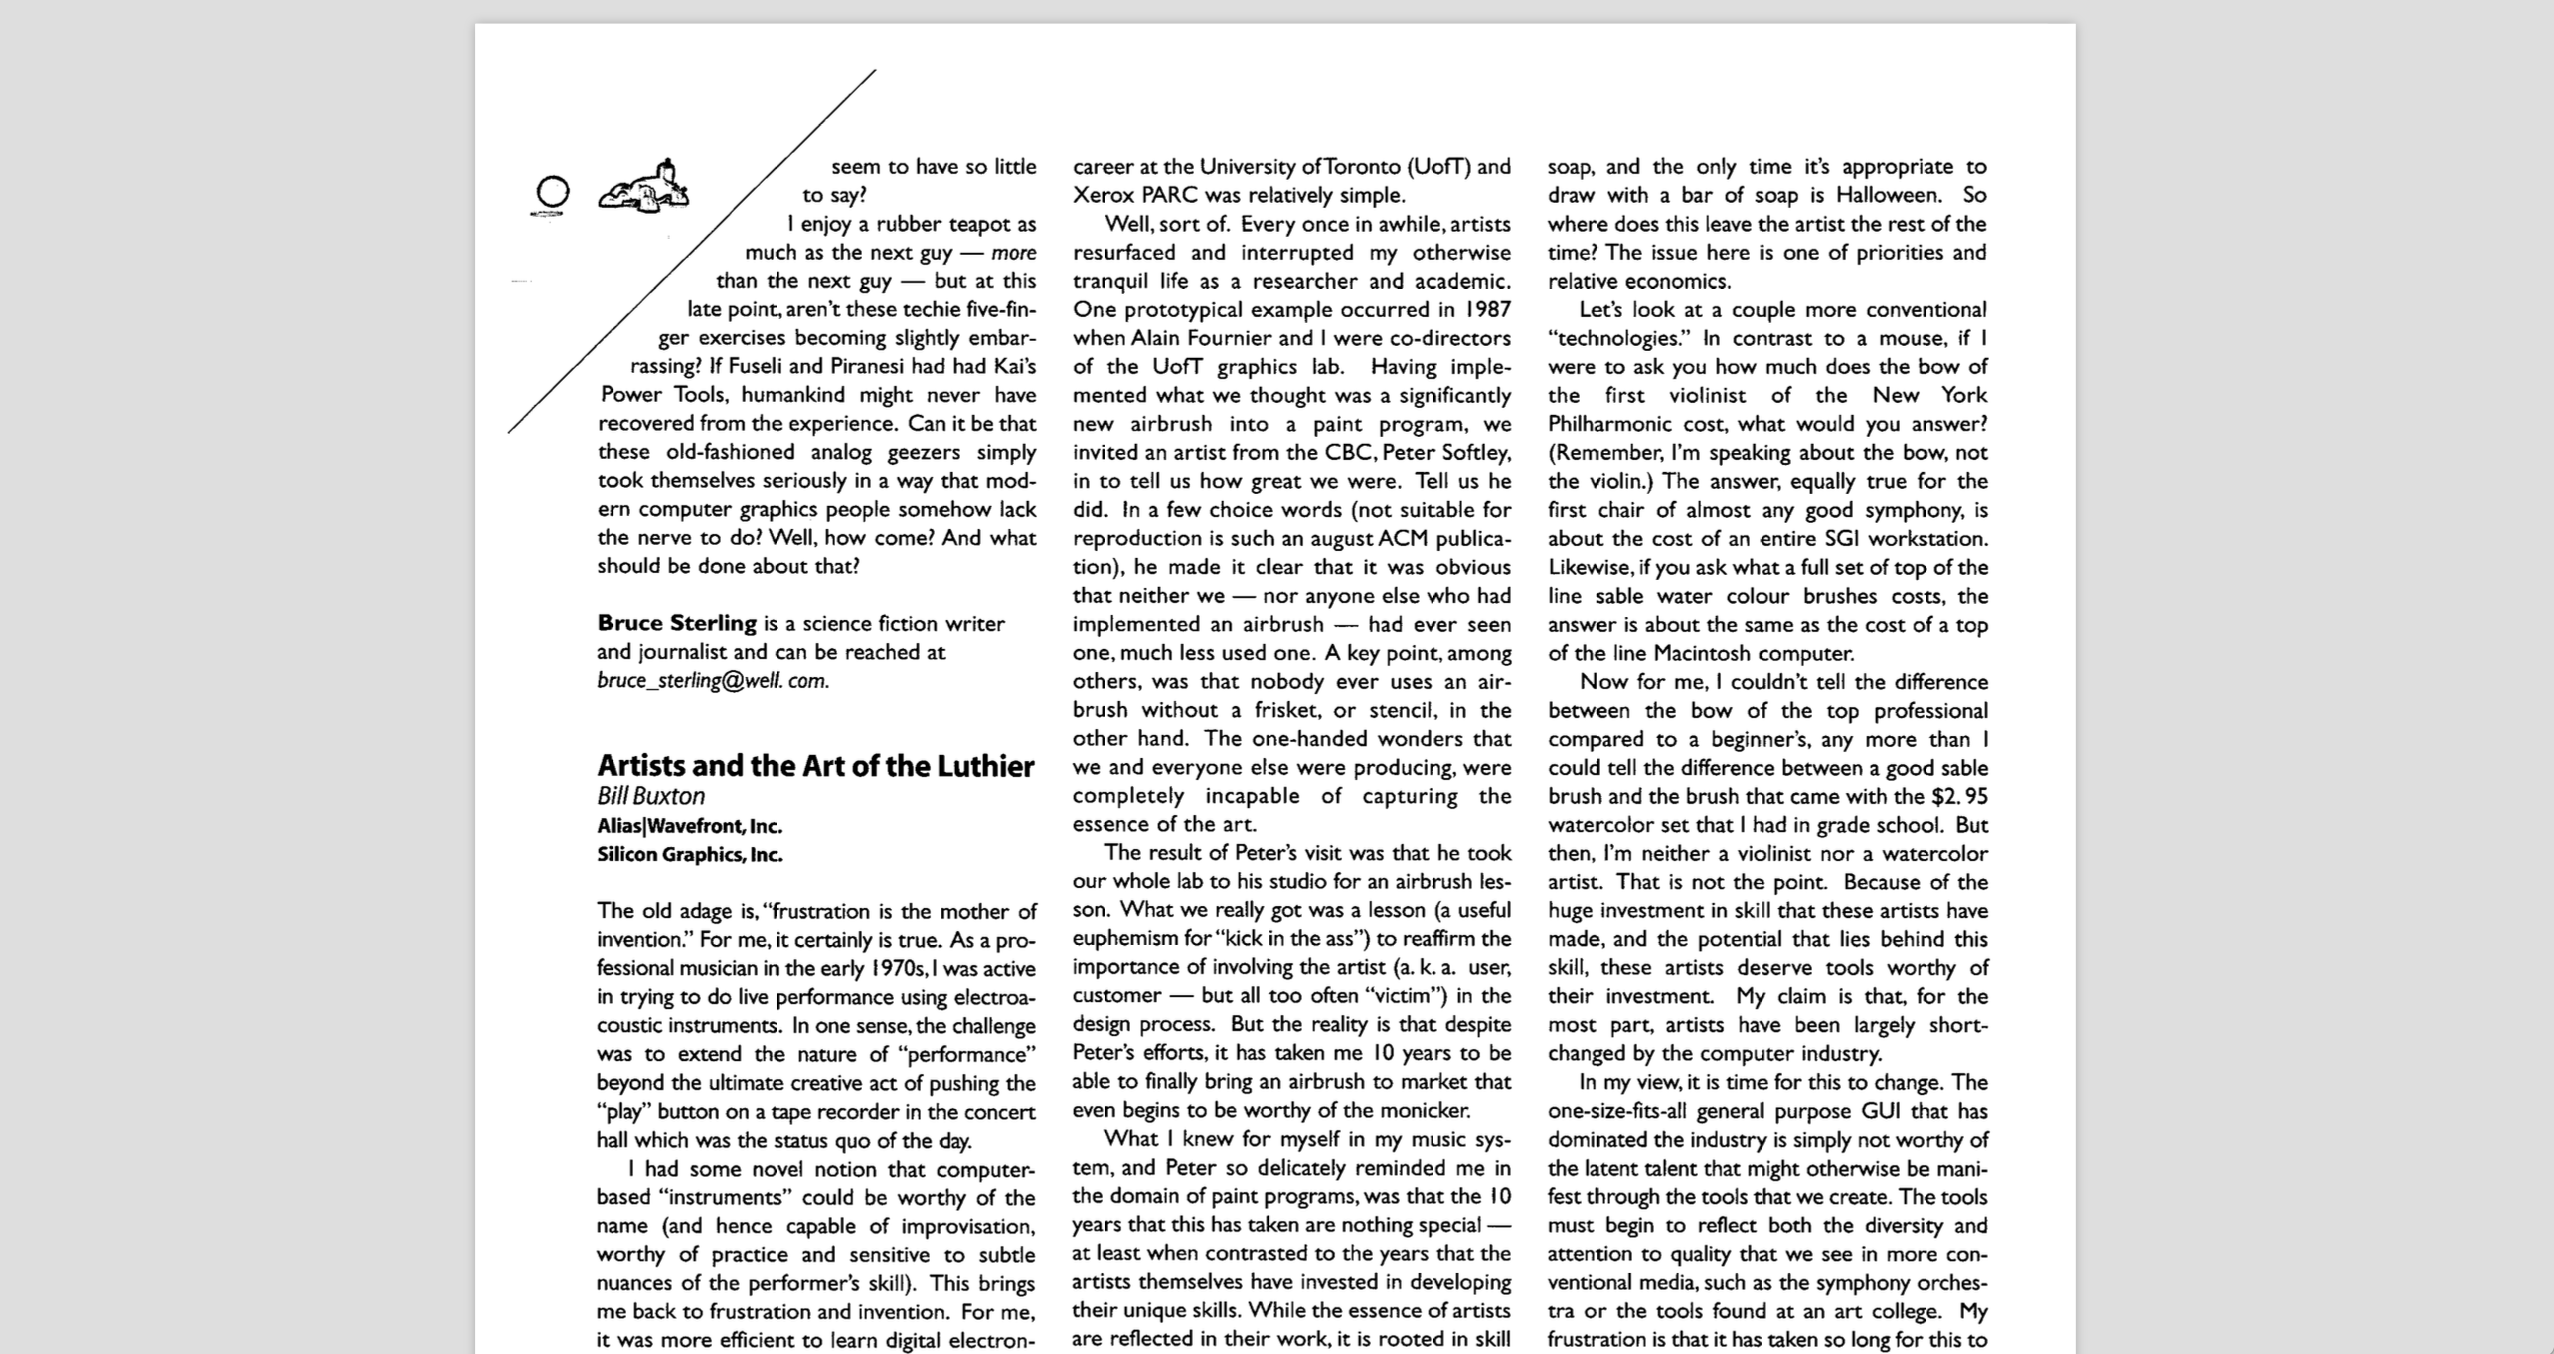
\includegraphics[scale=0.3]{img/Buxton-1997.png}\\
	    Buxton (1997) \cite{Buxton.1997.luthier}
    \end{figure}		
\end{frame}
%
\begin{frame}
\frametitle{}
\begin{figure}
	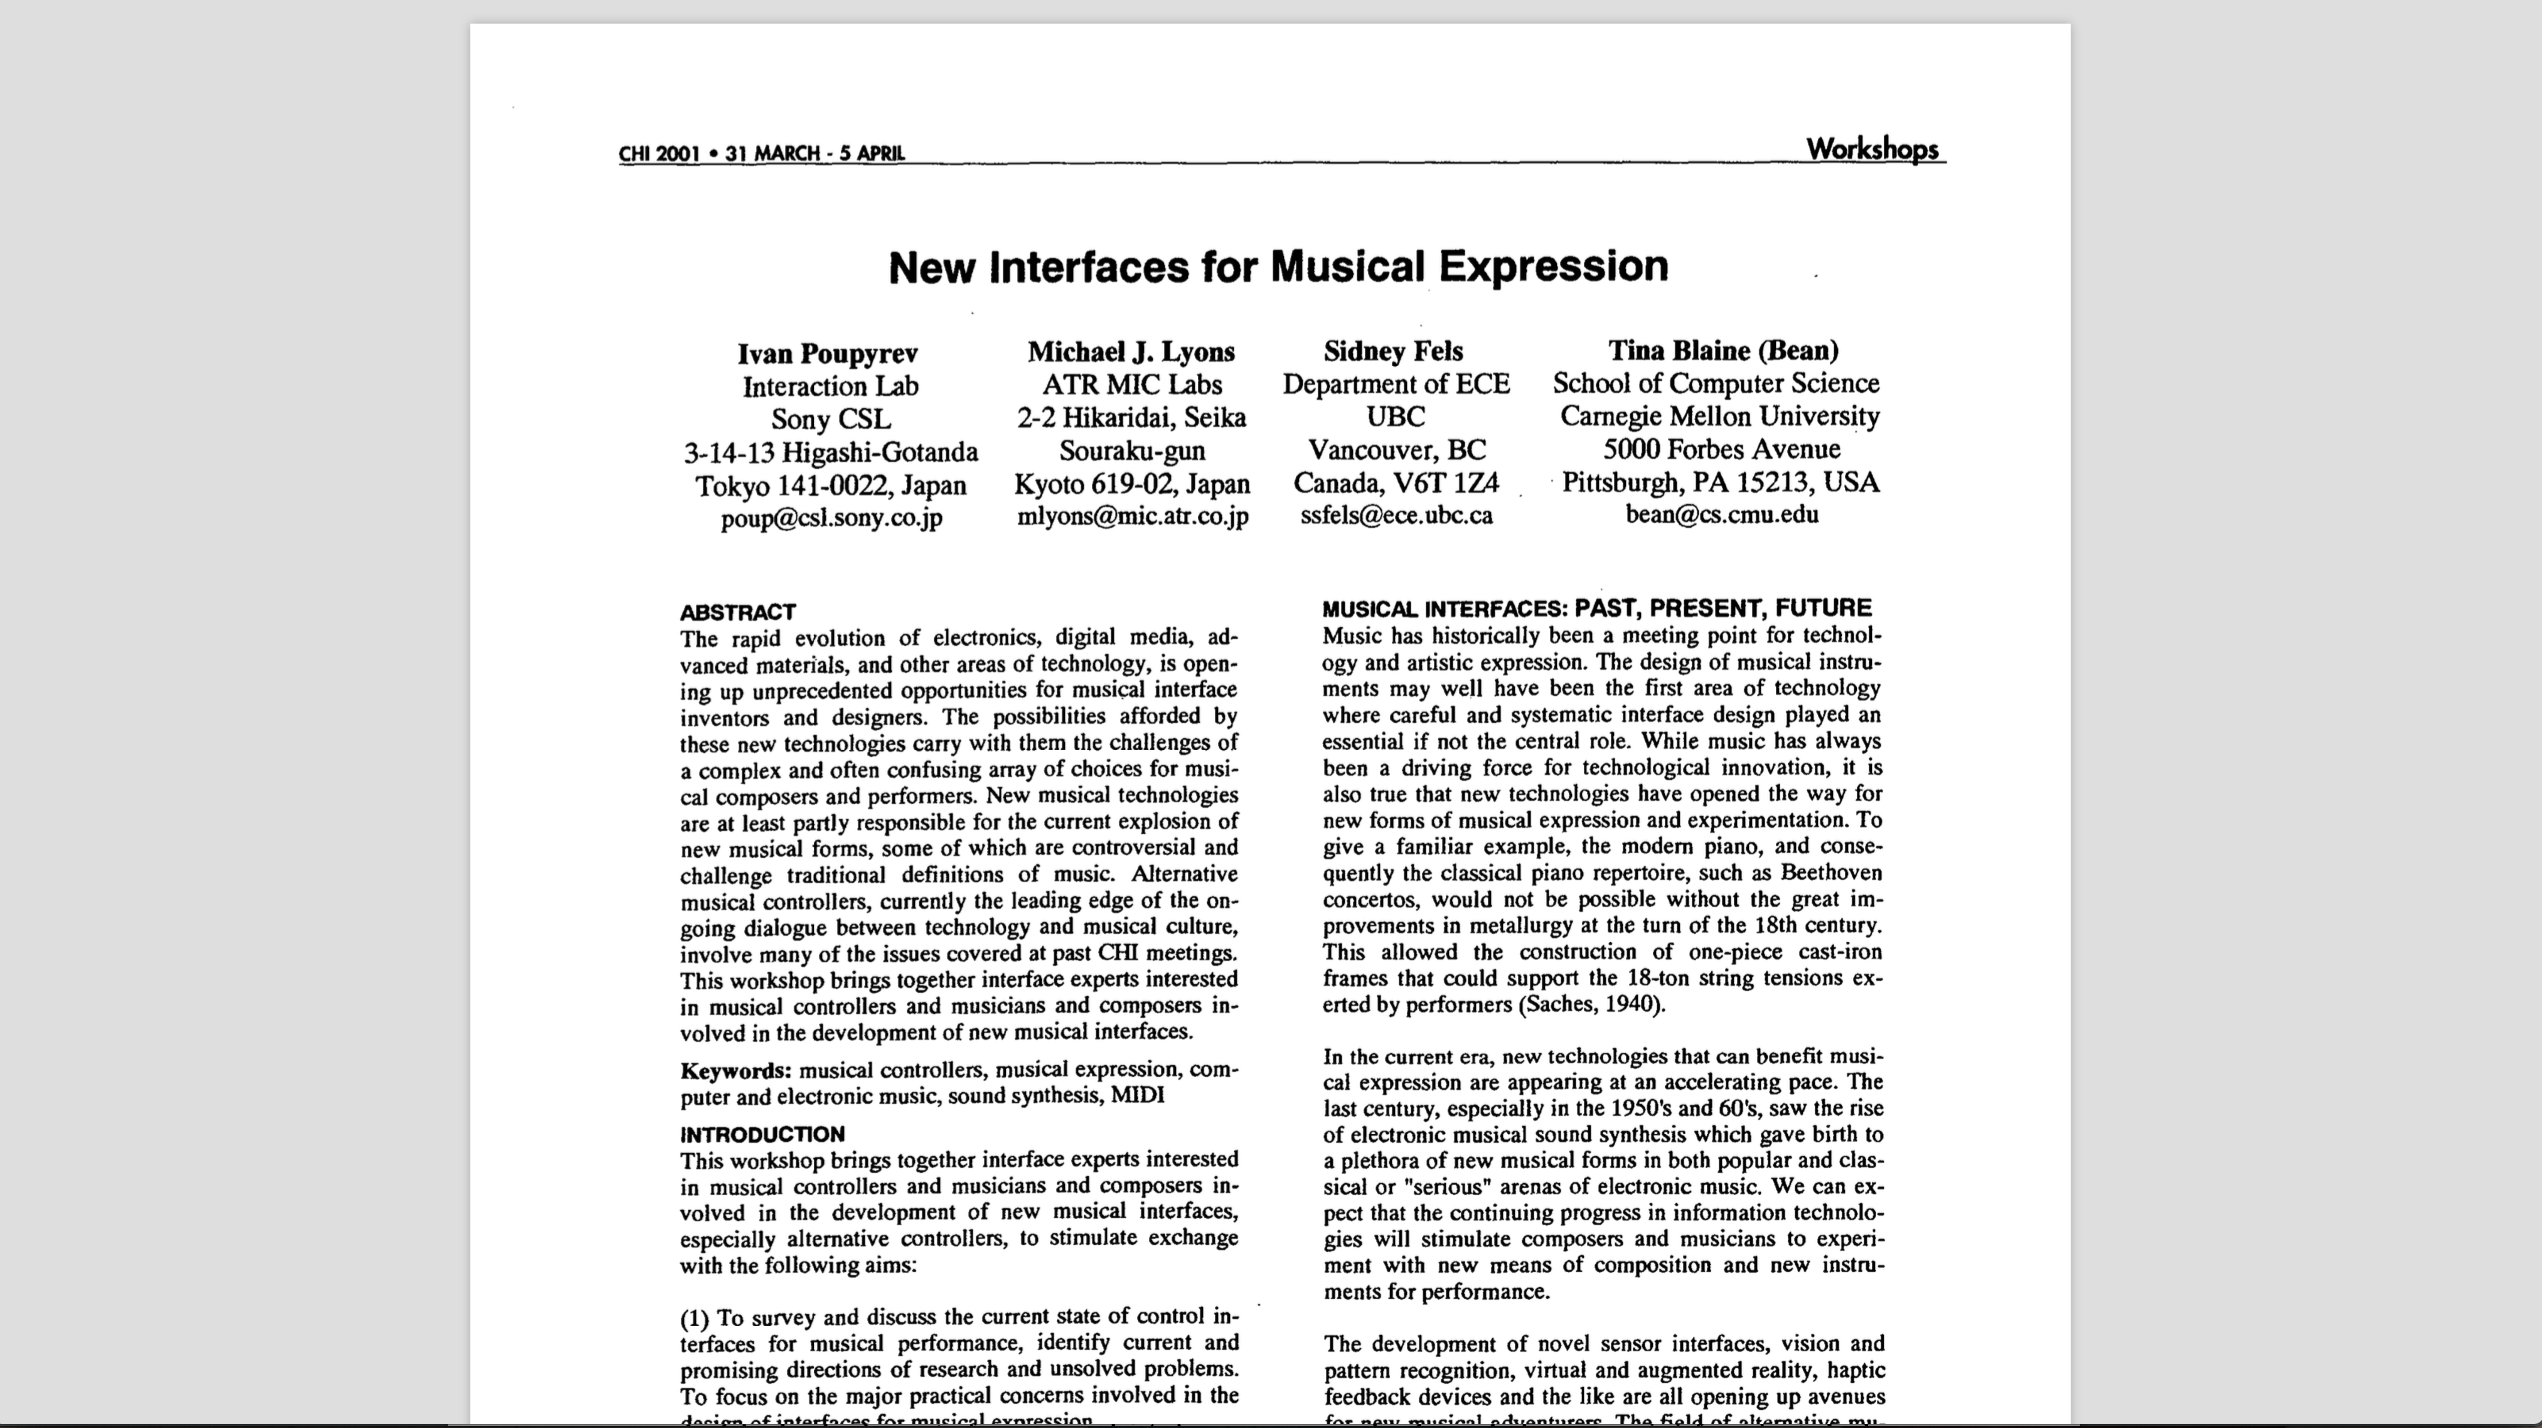
\includegraphics[scale=0.3]{img/Poupyrev-et-al-2001.png}\\
	    Pouprev et al. (2001) \cite{Poupyrev.et.al.2001}
    \end{figure}		
\end{frame}
%
\begin{frame}
\frametitle{Music and HCI (2013)}
\begin{figure}
	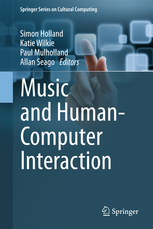
\includegraphics[scale=2.5]{img/Music-and-HCI.jpg}\\
	 Holland, S., Wilkie-McKenna, K., Mulholland, P., Seago, A. (Eds.) (2013) (\cite{Holland.et.al.2013}\\
	 Book URL: \url{https://www.springer.com/gb/book/9781447129899}
    \end{figure}		
\end{frame}
%
\begin{frame}
\frametitle{New Directions in Music and HCI (2019)}
\begin{figure}
	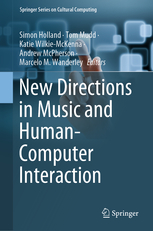
\includegraphics[scale=2.4]{img/New-Directions-Music-and-HCI.jpg}\\
	 Holland, S., Mudd, T., Wilkie-McKenna, K., McPherson, A., Wanderley, M. (Eds.) (\cite{Holland.et.al.2019}\\
	 Book URL: \url{https://www.springer.com/gp/book/9783319920689}
    \end{figure}		
\end{frame}
%
\begin{frame}
\frametitle{Other Resources and Perspectives}
\begin{itemize}
\item 120 Years of Electronic Music (1800--2019): \url{http://120years.net}
\item Sarah Reid, Sara Sithi-Amnuai, and Ajay Kapur. 2018. \emph{Women Who Build Things: Gestural Controllers, Augmented Instruments, and Musical Mechatronics}. \cite{Reid.et.al.2018.NIME}
\item Anna Xamb{\'o}. 2018. \emph{Who Are the Women Authors in NIME?--Improving Gender Balance in NIME Research}. \cite{Xambo.2018.NIME}
\item Adnan Marquez-Borbon and Juan Pablo Martinez-Avila. 2018. \emph{The Problem of DMI Adoption and Longevity: Envisioning a NIME Performance Pedagogy}. \cite{Marquez-Borbon.Martinez-Avila.2018.NIME}
\item Adnan Marquez-Borbon and Paul Stapleton. 2015. \emph{Fourteen Years of NIME: The Value and Meaning of `Community' in Interactive Music Research}. \cite{Marquez-Borbon.Stapleton.2015.NIME}
\end{itemize}
\end{frame}
%
\begin{frame}
\frametitle{We Need More HCI!}
\begin{figure}
	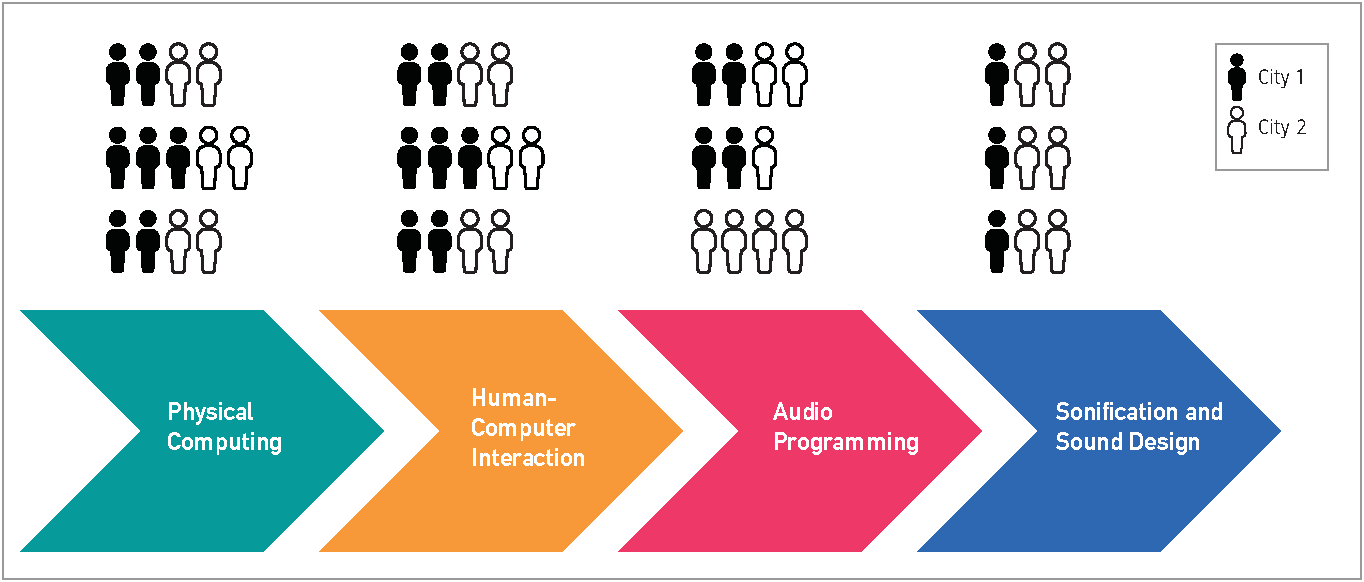
\includegraphics[scale=0.36]{img/timeline.pdf}\\
    \end{figure}
\begin{itemize}    
\item It is important to connect HCI more strongly with technological TBL courses related to prototyping interactive computer-based systems.
\item HCI can serve as a theoretical framework and critical-thinking tool.
\item This approach is helpful for shaping our future technological humanists as critical thinkers and agents of change.
\end{itemize}    
\end{frame}
%
\begin{frame}
\frametitle{}
\Huge{Survey time \& Closing}
\end{frame}
%
\begin{frame}
\frametitle{Human-Computer Interaction Day 4 - Group Assignment (post-class)}
\begin{itemize}
\item In this assignment, you are asked to create a diagram or a set of graphical representations of how the prototype that you built for the physical computing workshop works, focusing in the performance setting. This diagram should be included in the final assignment of writing a paper about the prototype. This assignment should be submitted before \textbf{Friday 1 November 2019 17:00}.
\item Assignment URL: \url{https://uio.instructure.com/courses/22318/assignments/28317}
\end{itemize}
\end{frame}
%
\begin{frame}
\frametitle{Human-Computer Interaction - Final Assignment}
\begin{itemize}
\item The final assignment of this course will consist in writing a short paper (2--4 pages long) about the prototype that you built in team and presented during the mini-hackathon of the Physical Computing Workshop. \textbf{Deadline: 8 November, 2019 @5pm}
\begin{itemize}
\item The individual part should include a link to a short video demonstrating your prototype. It is recommended to publish a blog post where the video is shortly introduced. In the paper the sections of ``Reflective notes'' and ``Conclusion'' should be individual.
\item The group part should write most of the paper together. It is a plus if you create a "short" version for the MCT blog, which should summarize the main points.
\item Assignment URL: \url{https://uio.instructure.com/courses/22318/assignments/28321}
\item Category for the blog post: \emph{HCI}, more info here: \url{https://github.com/MCT-master/mct-master.github.io} (README of the blog repo)
\end{itemize}
\end{itemize}
\end{frame}
%
\begin{frame}
\frametitle{Physical Computing Workshop\\ \small{Post-Questionnaire}}
\url{http://tiny.cc/pcw-postq}
\end{frame}
%
\begin{frame}
\frametitle{Experience in the Portal}
\url{http://tiny.cc/survey-portal}
\end{frame}
%
\begin{frame}[shrink=20]
  \frametitle{References}
  \printbibliography
\end{frame}
%
\end{document}
